\subsection{Admission inside a serving stack}
\label{sec:contract}
The additive bill charges a store as a constant paid by the request that creates the block. Whether the
request pays it depends on the connector's write path (\Cref{fig:conventions}c): LMCache's in-process connector
blocks each step until its saves to host memory complete, while vLLM's offloading connector submits them
asynchronously. We replayed slices of Alibaba's traceA (1,200 and 600 requests) and coder (600 requests), the
first third of each warming the caches, open-loop against vLLM 0.11 with the same model on one RTX A6000 (PCIe
Gen3), with a fresh server per run and one of three store rules sent with each request: store all, store
none, or a clairvoyant oracle that skips a request's store when it creates no block read again in the slice.
A 120\,GB host tier is large enough that storing everything and the oracle reach the same host hit ratio on
traceA; at 40\,GB storing everything crowds the tier. Before the runs we predicted that the oracle would lower
median time to first token (TTFT) by at least the store time it removes when the store blocks, more so under
heavier load, and by under 5\% when it does not unless the tier's hits change. Cells were repeated up to five
times in a shuffled order (\Cref{fig:contract}).

\begin{figure}[t]
  \centering
  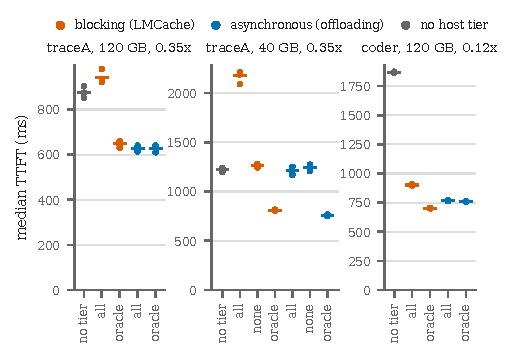
\includegraphics[width=\columnwidth]{fig_contract.pdf}
  \caption{Median TTFT of each replay run (one dot per run, bar at the mean) by write path and store rule:
  traceA with a 120\,GB and a 40\,GB host tier near saturation (0.35$\times$ the trace's arrival rate), and
  coder at a matched load. vLLM 0.11 on one RTX A6000; LMCache 0.3.9 blocks on its saves, vLLM's offloading
  connector does not.}
  \label{fig:contract}
\end{figure}

\noindent Both predictions held in every run. On traceA at 120\,GB, where the two rules' host hits agree
(11.3\% of tokens with one connector, 12.2\% with the other), the oracle lowers median TTFT by 31.1\% when the
store blocks and changes it by 0.3\% when it does not (18.0\% and 0.5\% at 0.2$\times$, five runs per cell); on
coder, where the oracle's host hits are three points higher, by 21.9\% and 1.3\%. With the same tier, storing
everything through the blocking path is 7.2\% slower than no host tier at all, through the asynchronous one
28.6\% faster. At 40\,GB storing everything adds 72.4\% over storing none when the store blocks and $-2.8$\%
when it does not, although its stores take 35.5\,ms per request; the oracle helps the asynchronous path there
too, through hits (1.9\% of tokens against 13.9\%), as a simulation of the tier had predicted. Against the
store time an additive bill charges, the blocking path pays 12 to 27 times as much near saturation and 1.4 to
1.7 times at 0.2$\times$: the excess is queueing. A causal rule that stores only prompts of at least 2,048
tokens lowers TTFT by 4.7\% on the blocking path and raises it by 6.0\% on the asynchronous one; by tokens, the
deployable rules we tried store nearly everything or nearly nothing. Medians can move more than means when
they fall between short and long prompts; under the mean every comparison keeps its sign, and the blocking
multiples near saturation are 11 to 28. The write path is one more convention an evaluation fixes, and it
decides whether admission matters. Per 512-token block this host stores in 8.3\,ms, loads from host memory in
5.5 and recomputes in 73.1, so under the additive price storing a new block pays above a 12.5\% chance that
it is read again.

\paragraph{A second engine} SGLang 0.5.10's hierarchical cache fixes its write path per server: write-through
stores each new block asynchronously when it is created, write-back stores a block, blocking, when it leaves the
GPU, and a selective write-through is documented to store a block on its second access. With the same GPU
pool, slice and loads, we predicted from a simulation of those semantics that the selective rule would store
almost nothing and act like no host tier; three of our four predictions failed. The engine counts a request's
own completion as a second access, so the selective rule stores every request that decodes more than one token,
and at 120\,GB all three rules cache 26.4\% of prompt tokens (14.3\% without the tier). What differs is
\emph{when}: storing at completion rather than at creation lowers median TTFT at 120\,GB and 0.35$\times$ by
22.6, 16.6 and 17.4\% in three runs (the mean by 8.8\% in each; the median by 3.8\% at 0.2$\times$), and the gap
persists with SGLang's direct transfers in place of its copy kernels, though both rules store asynchronously.
Profiling rules out contention between copies and prefill as the cause: under write-through 53 of 3{,}495
prefill kernels in a 60-second window overlapped a copy and ran twice as long, a few tens of milliseconds in
all; we did not find the cause. Blocking write-back costs 1.5\,ms at
0.35$\times$ and 20.5 at 0.2$\times$ at 120\,GB, against the growing penalty we predicted, but at 40\,GB and
0.35$\times$ it is slower than no hierarchical cache at all (827 against 653\,ms). A policy's name is not its
write path, and an asynchronous store is free on one engine and not on another.
